\section{MPTCP综述}
\subsection{背景}
随着技术的发展许多设备具有了多个网络接口,而TCP依然是一个单线路的协议,在TCP的通信过程中发端和收端都不能随意变换地址。我们可以利用多个网络接口的这一特性来改善性能和有效冗余。例如:你的手机同时连接WIFI信号和3G信号的时候(注意:这两个接口都是使用IP地址的,所以可以使用MPTCP,如果是蓝牙,没有IP地址,就不能使用MPTCP),如果WIFI关掉,使用WIFI进行的TCP连接就会断开,而不能有效利用3G网络继续收发数据。这里的问题还有一个很重要的意义就是在移动的网络中,需要切换地址的网络中有很重要的作用,清华现在正在做高铁上的MPTCP相关研究。MPTCP可以解决这些问题。

\subsection{简介}
MPTCP允许在一条TCP链路中建立多个子通道。当一条通道按照三次握手的方式建立起来后,可以按照三次握手的方式建立其他的子通道,这些通道以三次握手建立连接和四次握手解除连接。这些通道都会绑定于MPTCP session,发送端的数据可以选择其中一条通道进行传输。

\subsection{MPTCP设计原则}
MPTCP的设计遵守以下两个原则:
\begin{itemize}
	\item 应用程序的兼容性,应用程序只要可以运行在TCP环境下,就可以在没有任何修改的情况下,运行于MPTCP环境。{\color{red}{可能应用程序也需要进行MPTCP改造}}
	\item 网络的兼容性,MPTCP兼容其他协议。{\color{red}{我覺得MPTCP就是给TCP加了一层,所以所谓的兼容其他的协议,只是兼容TCP而已,因为它只使用TCP子流}}
\end{itemize}

\subsection{在协议栈中的位置}
在协议栈中的位置可以用图~\ref{label:MPTCP在协议栈中的位置}表示。
\begin{figure}[H]
	\centering
	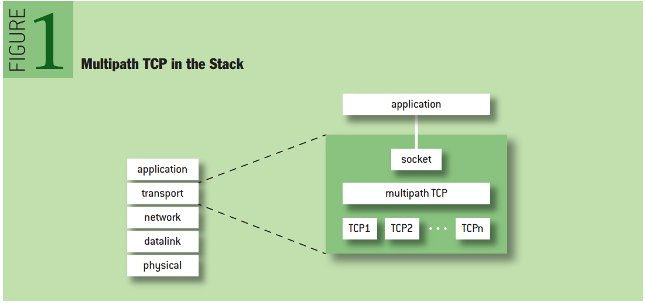
\includegraphics[width=10cm]{dias/MPTCP_position_in_protocol_stack.jpg}
	\caption{MPTCP在协议栈中的位置}
	\label{label:MPTCP在协议栈中的位置}
\end{figure}
在图中我们可以看到,其实MPTCP这一层算是重新搞出的一层,很明显增加了网络的复杂性,这必然会导致效率降低,如果它带来的提升不足以弥补这些负面效应,那也是没有意义的。具体怎么样,看看MPTCP1.0做得如何。